\documentclass[a4paper, 12pt, oneside, times, print, NoDraft]{template/UBtemplate}

%%
%% !!!! report mode
%%


%% parametre of UBtemplate

%%\documentclass[<Option1>, <Option2>, <Option3>, <Option4>, <Option5>, <Option6>,]{template/UBtemplate}
% <Option1>: page mode
% <Option2>: font size
% <Option3>: page side
% <Option4>: font style
% <Option5>: Print/Online Version
% <Option6>: Draft Option



% *************************** Page Options ******************************
% <a4paper> default size of the page
% <a5paper> secondary option for the size of the page
% *************************** Page Options ******************************



% ******************************* Font size Option ****************************
%<12pt> letter size at its standard 
%You can change the number (12) according to the size you want for your document.
% ******************************* Font size Option ****************************



% *************************** page side Options ******************************
%<oneside> (default) 
%<twoside>: Printing double side (twoside) or single side. Adds one blank page between pages.
% *************************** page side Options ******************************



% ******************************* Font Option **********************************
% <times> (default) : Times font with math support.

% <fourier>: Utopia Font with Fourier Math font (Font has to be installed)
%            It's a free font.

% <customfont>: Use `customfont' option in the document class and load the
% package in the preamble.tex
% ******************************* Font Option **********************************


% *********************** Define a Print/Online Version ************************
% <print>(default): Use `print' for print version with appropriate margins and page layout.

% <online> : activate Online version, the links won't have that blue color.
% *********************** Define a Print/Online Version ************************


% ****************************** Draft Option **********************************
% <NoDraft>(default): Special draft mode with line numbers, images, and water mark with timestamp and custom text. Position of the text can also be modified.

% <draft>: Special draft mode with line numbers, images, and water mark with
% timestamp and custom text. Position of the text can also be modified.
% ****************************** Draft Option **********************************

%% all packetge https://ctan.org/

%% tapa_cover
                                                                                                

%% units
\usepackage{siunitx}
\usepackage{ifthen}
\usepackage{ifpdf}


\usepackage{lscape}   % Supports Landscape Layout
\usepackage{setspace} % Define line spacing in paragraph
\usepackage{calc}     % calculate vertical spacing

% ************************* Conditional Statements *****************************
\usepackage{ifthen}   % Conditional statements
\usepackage{ifpdf}    % Check for pdfLaTeX
\usepackage{ifxetex}  % XeLaTeX
%% This will add the units
%----------------------------------------------
\newcommand{\nomunit}[1]{%
\renewcommand{\nomentryend}{\hspace*{\fill}#1}}
%----------------------------------------------


%% header & footer
\usepackage{fancyhdr} %% 页眉页脚 apply with geometry


%% nomenclatures Grouping
%% https://ctan.org/search?phrase=etoolbox
\usepackage{etoolbox}
\usepackage{makeidx}


%% nomenclatures package
%% ********************************************************* %%
%%                                                           %%
%%                       NOMENCLATURES                       %%
%%                                                           %%
%% ********************************************************* %%

%% https://www.overleaf.com/learn/latex/Nomenclatures
%% https://ctan.org/pkg/nomencl
\usepackage[intoc]{nomencl}


%-------------------------------Basic commands--------------------------------
\makenomenclature

% \nomenclature[⟨prefix ⟩]{⟨symbol⟩}{⟨description⟩}
% ⟨prefix ⟩ is used for fine tuning the sort order.
% ⟨symbol⟩ is the symbol you want to describe.
% ⟨description⟩ is the actual description.

% \printnomenclature 
% Put it at the place you want to have your nomenclature list.

%----------------------------------Referencing--------------------------------
% \nomrefeq % The phrase “, see equation (⟨eq⟩)” is appended to every entry in the nomenclature where ⟨eq⟩ is the number of the last equation in front of the corresponding command \nomenclature.

% \nomrefpage % Same as nomrefeq but for pages.

% \nomrefeqpage % Same as nomrefeq but for equations and pages

% \nomenclature{$a$}{The number of angels per unit area\nomrefeqpage}%
% \nomenclature{$N$}{The number of angels per needle point\nomrefeq}%
% \nomenclature{$A$}{The area of the needle point\nomrefeq\nomrefpage}%

% a The number of angels per unit area, see equation (1), page 1
% N The number of angels per needle point, see equation (1)
% A The area of the needle point, see equation (1), page 1

%------------------------Formatting Nomenclature------------------------------
% \printnomenclature % Change the label dimension,  you can use \printnomenclature[0.5in] instead of the simple \printnomenclature.

% \nomname % In case you don’t like the name of the nomenclature, just redefine the \nomname, e.g. \renewcommand{\nomname}{List of Symbols}

% \nomgroup % same as nomname but for group

% \nompreamble % same as nomname but for preamble

% \nomitemsep % adjust the skip between two entries

% \nomprefix  % redifine  the default prefix that is used for the sortkeys




%% glossaries package
%% ********************************************************* %%
%%                                                           %%
%%                       Glossaries                          %%
%%                                                           %%
%% ********************************************************* %%

%% https://www.overleaf.com/learn/latex/Glossaries
%% https://ctan.org/pkg/glossaries
\usepackage[toc]{glossaries}

\makeglossaries

%% appendix

%% https://ctan.org/pkg/appendix
\usepackage{appendix}

%% Bibliography
%% ********************************************************* %%
%%                                                           %%
%%                       Bibliography                        %%
%%                                                           %%
%% ********************************************************* %%



\usepackage[
    backend=biber,
    style=alphabetic,
    sorting=ynt
]{biblatex}



\addbibresource{optional/bibliography/bibliography.bib}


%% indices of terms:
%% ********************************************************* %%
%%                                                           %%
%%                       INDICES OF TERMS                    %%
%%                                                           %%
%% ********************************************************* %%


%% https://ctan.org/pkg/imakeidx
\usepackage{imakeidx}
\makeindex[title=Alphabetical Index, columns=3,  columnsep=2cm, intoc]
%% More detaill about \makeindex[<parameters >] please to see file <optional/indices_of_terms.tex>


%% \makeindex[]
%% Parameters for the \makeindex command:
%% \makeindex[
%% title=<contents>,
%% columns=<number>,
%% columnsep=<number unit>,
%% intoc,
%% columnseprule
%% ]

%% title         : The default contents is 2, Title to be typeset at the beginning of the specific index. An example is presented in formatting the index.
%%
%% columns       : The default value is 2, Uses the syntax key=value, the value must be an integer representing the number of columns. 
%%
%% columnsep     : Specifies units that represent the separation between the columns. The syntax must be key=value, for example columnsep=2em.
%%
%% intoc         : If this option is passed, the index title is put in the table of contents. 
%%
%% columnseprule : If option is passed, a vertical ruler will be rendered between the column

\renewcommand\thesection{\arabic{section}}


%% 几乎必须
\usepackage{amsmath}  %%数学公式
\usepackage{graphicx} %%插图 
\usepackage{xcolor}   %%颜色 
\usepackage{array}    %%表格 

%% 样式定制
\usepackage{geometry} %%页面布局
\usepackage{titlesec} %%页眉页脚
\usepackage{enumitem} %%列表 
\usepackage{footmisc} %%脚注 
\usepackage{listings} %%抄录环境 
\usepackage{amsthm}   %%定理环境
\usepackage{thmtools} %%定理环境


%% 特定领域
\usepackage{amssymb}  %%更多公式符号
\usepackage{ragged2e} %%段落对齐方式




\usepackage[utf8]{inputenc}

\usepackage{setspace}


%% 中文

% 页眉和页脚
\usepackage{fancyhdr}


\usepackage{mathtools}
\usepackage{amsmath, amssymb, amsthm}
\usepackage{enumerate, enumitem}

\usepackage{fancyhdr, graphicx, proof, comment, multicol}
\usepackage[none]{hyphenat}
\usepackage{dirtytalk}
\binoppenalty=\maxdimen
\relpenalty=\maxdimen
\usepackage{microtype}
%\usepackage{mathpazo}
\usepackage{mdframed}
\usepackage{parskip}
\linespread{1}
\usepackage{subfig}
\usepackage{mathrsfs}
\usepackage{hyperref}
\usepackage{amsfonts}
\usepackage{minted}
\usepackage{amssymb}
\usepackage{algorithm}
\usepackage{ragged2e}
\usepackage[noend]{algpseudocode}
\usepackage{hyperref}



\newtheorem{defn0}{Definition}[section]
\newtheorem{prop0}[defn0]{Proposition}
\newtheorem{thm0}[defn0]{Theorem}
\newtheorem{lemma0}[defn0]{Lemma}
\newtheorem{corollary0}[defn0]{Corollary}
\newtheorem{example0}[defn0]{Example}
\newtheorem{remark0}[defn0]{Remark}
\newtheorem{conjecture0}[defn0]{Conjecture}

\newenvironment{definition}{ \begin{defn0}}{\end{defn0}}
\newenvironment{proposition}{\bigskip \begin{prop0}}{\end{prop0}}
\newenvironment{theorem}{\bigskip \begin{thm0}}{\end{thm0}}
\newenvironment{lemma}{\bigskip \begin{lemma0}}{\end{lemma0}}
\newenvironment{corollary}{\bigskip \begin{corollary0}}{\end{corollary0}}
\newenvironment{example}{ \begin{example0}\rm}{\end{example0}}
\newenvironment{remark}{ \begin{remark0}\rm}{\end{remark0}}
\newenvironment{conjecture}{\begin{conjecture0}}{\end{conjecture0}}

\newcommand{\defref}[1]{Definition~\ref{#1}}
\newcommand{\propref}[1]{Proposition~\ref{#1}}
\newcommand{\thmref}[1]{Theorem~\ref{#1}}
\newcommand{\lemref}[1]{Lemma~\ref{#1}}
\newcommand{\cororef}[1]{Corollary~\ref{#1}}
\newcommand{\exref}[1]{Example~\ref{#1}}
\newcommand{\secref}[1]{Section~\ref{#1}}
\newcommand{\remref}[1]{Remark~\ref{#1}}
\newcommand{\conjref}[1]{Conjecture~\ref{#1}}
\DeclarePairedDelimiterX{\norm}[1]{\lVert}{\rVert}{#1}

\usemintedstyle{vs}

\addtolength{\topmargin}{-10.54448pt}







\usepackage{graphicx}
\graphicspath{{./preambles/static/ub_logo}}     %% ub logo
\graphicspath{{./images/}}                      %% upload images
\usepackage{listings}
\usepackage{xcolor}

\lstdefinestyle{DOS} {
    backgroundcolor = \color{black},
    basicstyle = \color{white} \scriptsize \ttfamily
}

% Add non UTF-8 characters

\lstset{
     literate =
         {á}{{\'a}}1
         {í}{{\'i}}1
         {é}{{\'e}}1
         {ý}{{\'y}}1
         {ú}{{\'u}}1
         {ó}{{\'o}}1
         {ě}{{\v{e}}}1
         {š}{{\v{s}}}1
         {č}{{\v{c}}}1
         {ř}{{\v{r}}}1
         {ž}{{\v{z}}}1
         {ď}{{\v{d}}}1
         {ť}{{\v{t}}}1
         {ň}{{\v{n}}}1                
         {ů}{{\r{u}}}1
         {Á}{{\'A}}1
         {Í}{{\'I}}1
         {É}{{\'E}}1
         {Ý}{{\'Y}}1
         {Ú}{{\'U}}1
         {Ó}{{\'O}}1
         {Ě}{{\v{E}}}1
         {Š}{{\v{S}}}1
         {Č}{{\v{C}}}1
         {Ř}{{\v{R}}}1
         {Ž}{{\v{Z}}}1
         {Ď}{{\v{D}}}1
         {Ť}{{\v{T}}}1
         {Ň}{{\v{N}}}1
         {Ů}{{\r{U}}}1
}



% The emptypage package prevents page numbers and
% headings from appearing on empty pages.
\usepackage{emptypage}

\usepackage{booktabs} % For professional looking tables
\usepackage{multirow}
\begin{document}



%% ******************* Personal zone ******************* %%
%You can change your cover and footer style
% ******************************** Title Page **********************************


\title{My Title}
\subtitle{My Subtitle}
\author{Author 1, Author 2}
\dept{Department of Mathematics and Computer Science}
\university{University of Barcelona}

\crest{
\includegraphics[width=0.2\textwidth]{preambles/static/ub_logo/ub_logo_3.png}}

\supervisor{Prof. A.B. \newline
            Prof. C.D. }
            
\advisor{Dr. A. Advisor\newline 
         Dr. B. Advisor}
\renewcommand{\submissiontext}{change the default text here if needed, or delete it}
\degreetitle{Doctor of Computer Science}
\college{Computer Science}
\degreedate{Desembre 2022}

\subject{LaTeX} \keywords{{LaTeX} {Thesis} {Engineering} {University of Barcelona}}


%% make title
\maketitle
%% tutotrial of page numbering: https://www.overleaf.com/learn/latex/Page_numbering
%% \pagenumbering{<numberstyle>}
%% <numberstyle>:
%% <arabic> : use Arabic numerals (1, 2, 3, ...)
%% <alph>   : use lowercase letters (a, b, c, ...)
%% <Alph>   : use uppercase letters (A, B, C, ...)
%% <roman>  : use lowercase roman numerals (i, ii, iii, ...)
%% <Roman>  : use uppercase roman numerals (I, II, III, ...)

%% \frontmatter : Pages after this command and before the command \mainmatter, 
%%                will be numbered with lowercase Roman numerals.
%% \mainmatter  : This will restart the page counter and change the style to Arabic numbers.



%% tutotrial of headers and footers: https://www.overleaf.com/learn/latex/Headers_and_footers

%% \pagestyle{<style>}    : sets the style of the current page, and all subsequent pages, to <style>
%% \thispagestyle{<style>}: sets style of the current page only to <style>
%% style:
%% <empty>      : no headers or footers on pages
%% <plain>      : no page headers, footers consist of a centered page number
%% <headings>   : no footers, headers contains class-specific information and page number
%% <myheadings> : no footers, headers contains page number and user-supplied information
%% <package>    : use the specified package


%% \usepackage[⟨options⟩]{fancyhdr}
%% \pagestyle{fancyhdr}
%% \fancyhf[locations]{content}
%% [locations]:
%% O - E     : to specify Odd or Even pages
%% H - F     : to indicate Header or Footer
%% L - C - R : for the Left, Centre and Right “zone” of the header or footer


%% \headrulewidth : macro to define the thickness of a line under the header
%% \footrulewidth : macro to define the thickness of a line above the footer
%% \headruleskip  : macro to define the distance between the line and the header text (only available since version 4.0)
%% \footruleskip  : macro to define the distance between the line and the footer text
%% \headrule      : macro to completely redefine header rules (lines)
%% \footrule      : macro to completely redefine footer rules (lines)
%% \headwidth     : a length parameter that defines the total width of the headers and footers


%% \usepackage{fancyhdr}
%%\pagestyle{fancy}

%%\fancyhf{}
%%\fancyhf[EHL]{eqweqw}
%%\fancyhf[EHC]{eqweqw}
%%\fancyhf[EHR]{eqweqwe}


%%\fancyhf[OFL]{\thepage}
%%\fancyhf[OFC]{\thepage}
%%\fancyhf[OFR]{\thepage}


% Style 1: Sets Page Number at the Top and Chapter/Section Name on LE/RO
\fancypagestyle{PageStyle1}{
  \renewcommand{\chaptermark}[1]{\markboth{##1}{}}
  \renewcommand{\sectionmark}[1]{\markright{\thesection\ ##1\ }}
  
  \fancyhf{}
  \fancyhead[RO]{\nouppercase \rightmark\hspace{0.25em} | 
    \hspace{0.25em} \bfseries{\thepage}}
  \fancyhead[LE]{ {\bfseries\thepage} \hspace{0.25em} | 
    \hspace{0.25em} \nouppercase \leftmark}
}

% Style 2: Sets Page Number at the Bottom with Chapter/Section Name on LO/RE
\fancypagestyle{PageStyle2}{
  \renewcommand{\chaptermark}[1]{\markboth{##1}{}}
  \renewcommand{\sectionmark}[1]{\markright{\thesection\ ##1}}
  \fancyhf{}
  \fancyhead[RO]{\bfseries\nouppercase \rightmark}
  \fancyhead[LE]{\bfseries \nouppercase \leftmark}
  \fancyfoot[C]{\thepage}
}

%Default Style: Sets Page Number at the Top (LE/RO) with Chapter/Section Name
\fancypagestyle{PageStyle3}{
    \renewcommand{\chaptermark}[1]{\markboth {##1}{}}
    \renewcommand{\sectionmark}[1]{\markright{\thesection\ ##1}}
    \fancyhf{}
    \fancyhead[LO]{\nouppercase \rightmark}
    \fancyhead[LE,RO]{\bfseries\thepage}
    \fancyhead[RE]{\nouppercase \leftmark}
}

\setlength{\headheight}{14.5pt}

\pagestyle{PageStyle3}
%% ******************* Personal zone ******************* %%


\frontmatter %Use lowercase Roman numerals for page numbers


%-----------------------ALL OPTIONAL ZONE CAN BE DELETED--------------------------
%% ******************* optional zone ******************* %%

% ********************************* Dedication *********************************
% The dedication environment makes sure the dedication gets its
% own page, centered
\newenvironment{dedication}{
    \clearpage % \cleardoublepage
    \setsinglecolumn
    \vspace*{0.2\textheight}
    \thispagestyle{empty}
    \centering
}




\begin{dedication} 




I would like to dedicate this thesis to my loving parents ...




\end{dedication}



% ******************************* Declaration **********************************
% The declaration environment puts a large, bold, centered
% "Declaration" label at the top of the page.
\newenvironment{declaration}{
    \clearpage % \cleardoublepage
    \setsinglecolumn
    
    \addcontentsline{toc}{chapter}{Declaration}
    \chapter*{\centering \Large Declaration}
    
    \thispagestyle{plain}
}



%{
%    \flushright
%    \@author{}\\
%    \@degreedate{}
%    \vfill
%}


\begin{declaration}



I hereby declare that ...




\end{declaration}
% ****************************** Acknowledgements ********************************
% The acknowledgements environment puts a large, bold, centered
% "Acknowledgements" label at the top of the page.

\newenvironment{acknowledgements}{
    \clearpage %\cleardoublepage
    \setsinglecolumn
    
    \addcontentsline{toc}{chapter}{Acknowledgements}
    \chapter*{\centering \Large Acknowledgements}
    
    \thispagestyle{plain}
}




\begin{acknowledgements}






And I would like to acknowledge ...







\end{acknowledgements}
% To include only the Title and the abstract pages for submission to BoGS

    %\renewcommand{\tableofcontents}{}
    %\renewcommand{\listoffigures}{}
    %\renewcommand{\listoftables}{}
    %\renewcommand{\printnomencl}{}
    %\renewcommand{\printnomencl}[1][2]{}
    %\renewcommand{\printthesisindex}{}
    %\renewcommand{\bibname}{}
    %\renewcommand{\bibliography}[1]{\thispagestyle{empty}}

% ******************************** Abstract ************************************
% The abstract environment puts a large, bold, centered "Abstract" label at
% the top of the page. Defines both abstract and separate abstract environment
\newenvironment{abstract} {
  \clearpage %\cleardoublepage
  \setsinglecolumn
  
  \addcontentsline{toc}{chapter}{Abstract}
  \chapter*{\centering \Large Abstract}
  
  \thispagestyle{plain}
}


\begin{abstract}




This is where you write your abstract ...





\end{abstract}

%% tutorial table_of_contents:
%% https://www.overleaf.com/learn/latex/Table_of_contents


%% \renewcommand*\contentsname{content} %% content --> you can replace whatever you want


\renewcommand*\contentsname{Contents} 


\tableofcontents


\mainmatter % Now Use Arabic numerals for page numbers


\newglossaryentry{latex}
{
    name=latex,
    description={Is a markup language specially suited 
    for scientific documents}
}

\newglossaryentry{maths}
{
    name=mathematics,
    description={Mathematics is what mathematicians do}
}








\clearpage
\printglossaries[intoc]

%% Nomenclatures
%% tutorial && example:
%% https://www.overleaf.com/learn/latex/Nomenclatures
%% https://ctan.org/pkg/nomencl

%%----------------------------------LIST--------------------------------------
\renewcommand{\nomname}{List of Symbols}
%% \renewcommand{\nomname}{<contents>} : <contents> --> changes the default title.


\renewcommand{\nompreamble}{The next list describes several symbols that will be later used within the body of the document}
%% \renewcommand{\nompreamble}{<contents>} : <contents> --> inserts some text in between the title and the list symbols.

%%---------------------------------GROUP--------------------------------------

%% https://ctan.org/pkg/etoolbox
\renewcommand\nomgroup[1]{
  \item[\bfseries
  \ifstrequal{#1}{A}{Physics constants}{
  \ifstrequal{#1}{B}{Number sets}{
  \ifstrequal{#1}{C}{Other symbols}}}
  %% ... same example just like before
]}


\nomenclature[A, 02]{\(c\)}{Speed of light in a vacuum\nomunit{\SI{299792458}{\meter\per\second}}}

\nomenclature[A, 03]{\(h\)}{{Planck constant}\nomunit{\SI[group-digits=false]{6.62607015e-34}{\joule\per\hertz}}}

\nomenclature[A, 01]{\(G\)}{{Gravitational constant} \nomunit{\SI[group-digits=false]{6.67430e-11}{\meter\cubed\per\kilogram\per\second\squared}}}

\nomenclature[B, 03]{\(\mathbb{R}\)}{Real numbers}
\nomenclature[B, 02]{\(\mathbb{C}\)}{Complex numbers}
\nomenclature[B, 01]{\(\mathbb{H}\)}{Quaternions}

\nomenclature[C]{\(V\)}{Constant volume}
\nomenclature[C]{\(\rho\)}{Friction index}

%%\nomenclature[<prefix>]{<symbol>}{<description>}
%% <prefix>      : is used for fine tuning the sort order.
%% <symbol>      : is the symbol you want to describe.
%% <description> : is the actual description of than symbol.

%%\usepackage{ifthen}
%\renewcommand{\nomgroup}[1]{%
%  \item[\bfseries
%  \ifthenelse{\equal{#1}{P}}{Physics constants}{%
%  \ifthenelse{\equal{#1}{O}}{Other symbols}{%
%  \ifthenelse{\equal{#1}{N}}{Number sets}{}}}%
%  %%compare the first two arguments, if they are equal the term is added to the group, otherwise the %next nested condition is checked.
%]}


\clearpage
\printnomenclature
%% ******************* optional zone ******************* %%


\chapter{Getting started}

\section{An Introduction}
This template was created by Junjie Li, the primary contributor, and Manuel Liu Wang, the secondary contributor, both UB students majoring in computer science. It is not an official template from UB.

It can be an essay, thesis, report, or article. The template is for broad usage. Mathematical notation, matrix application, pictures, formulas, a range of word styles, and page size are all included.


\section{Tutorial}
Options \underline{[Option1, Option2, Option3, Option4, Option5, and Option6]} are listed in the first line. , those options regulate the template's fundamental layout: Option 1 modifies the page mode; Option 2 sets the font size; Option 3 establishes the page side; Option 4 applies the desired font style; Option 5 toggles the print/online version; and Option 6 activates the draft option.

On the other side, there is the optional zone, which you can omit if you choose. For instance, the first optional zone has the cover and the footer.


\section{Usage}

You can look at the chapter sections, beginning with section 2, to get a quick overview of how to use this template. All the chapters have usage examples.    




\chapter{My second Chapter}

\section{Images exemple}


\textbf{Example of an image:}
\begin{figure}[H]
    \centering
    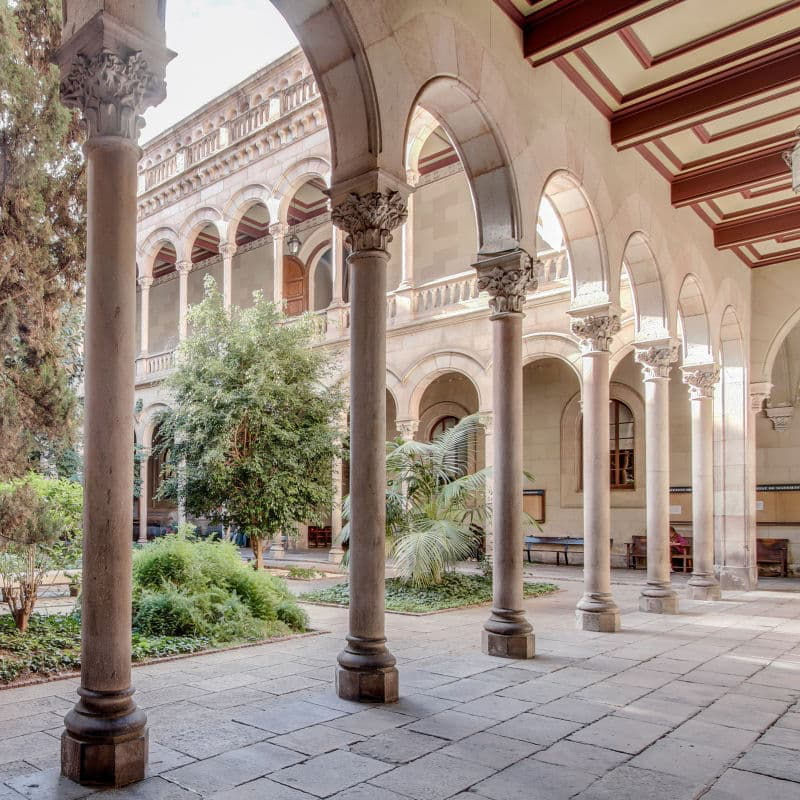
\includegraphics[width=6cm, height=4cm]{images/edifici-historic-universitat-de-barcelona.jpg}
    \caption{Image example}
    \label{fig:image_example}
\end{figure}

\textbf{Example of an image without caption:}
\begin{figure}[H]
    \centering
    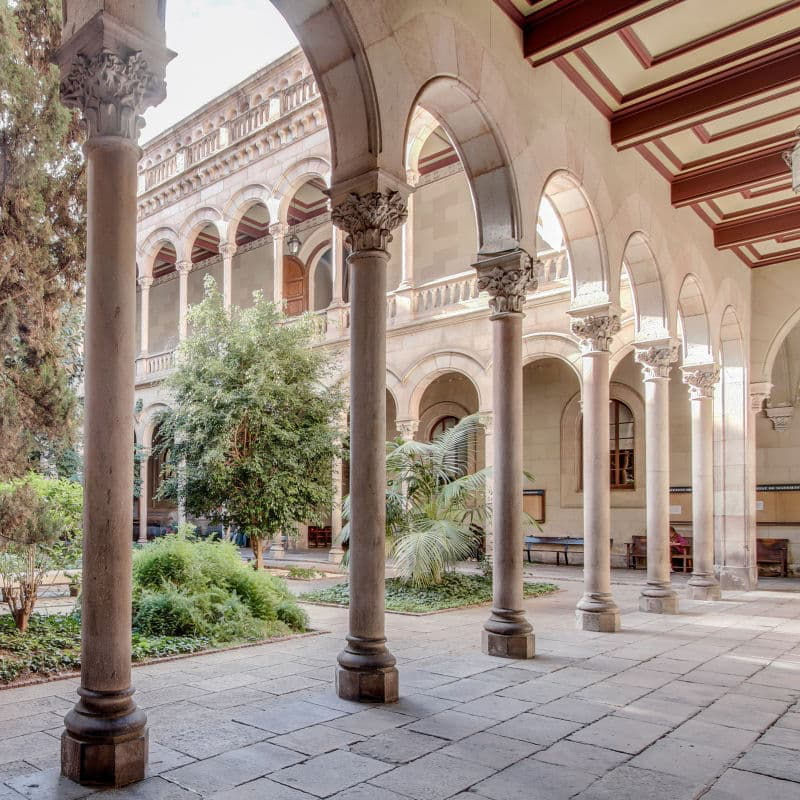
\includegraphics[width=6cm, height=4cm]{images/edifici-historic-universitat-de-barcelona.jpg}
    \label{fig:image_example_no_caption}
\end{figure}


\textbf{Example of two images:}
\begin{figure}[H]
    \centering
    \begin{minipage}[t]{0.48\textwidth}
        \centering
        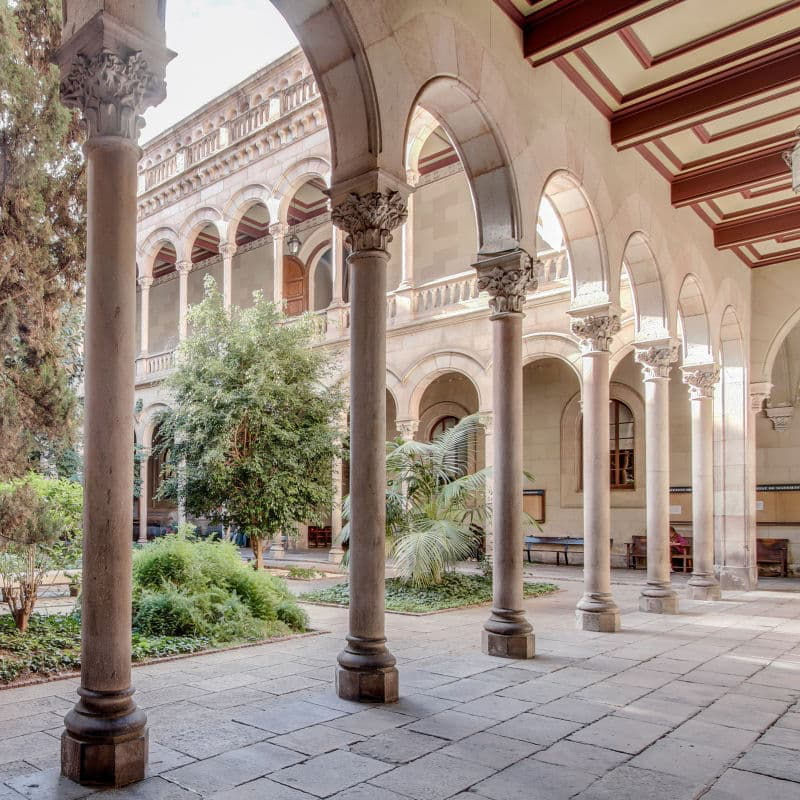
\includegraphics[width=6cm, height=4cm]{images/edifici-historic-universitat-de-barcelona.jpg}
        \caption{Image example2}
        \label{fig:image_example2}
    \end{minipage}
    \begin{minipage}[t]{0.48\textwidth}
        \centering
        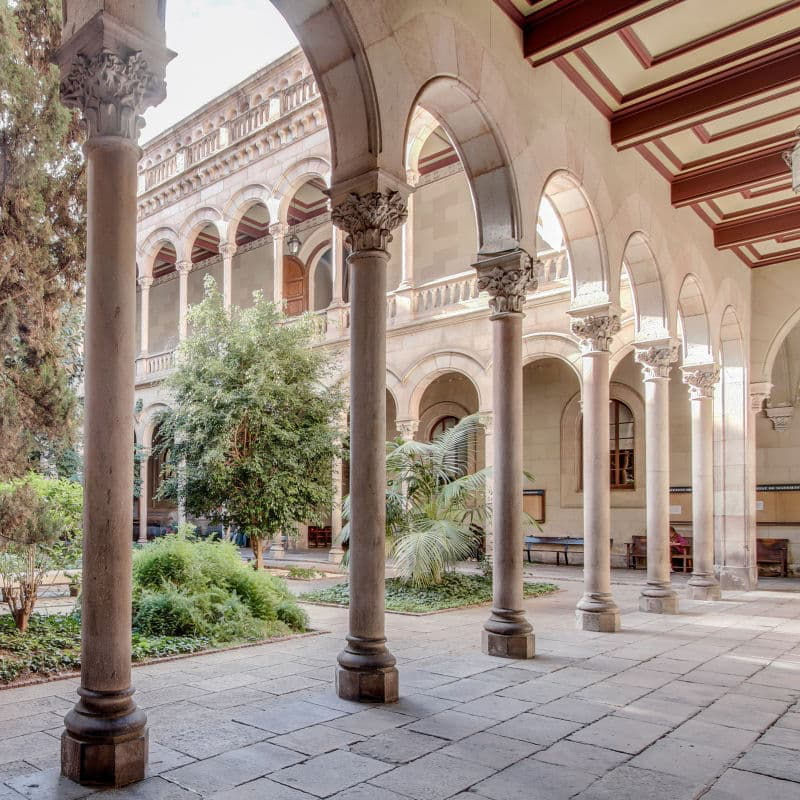
\includegraphics[width=6cm, height=4cm]{images/edifici-historic-universitat-de-barcelona.jpg}
        \caption{Image example3}
        \label{fig:image_example3}
    \end{minipage}
\end{figure}



\textbf{Example of two images with one caption:}
\begin{figure}[h]
  \centering
  \begin{minipage}{0.45\textwidth}
    \centering
    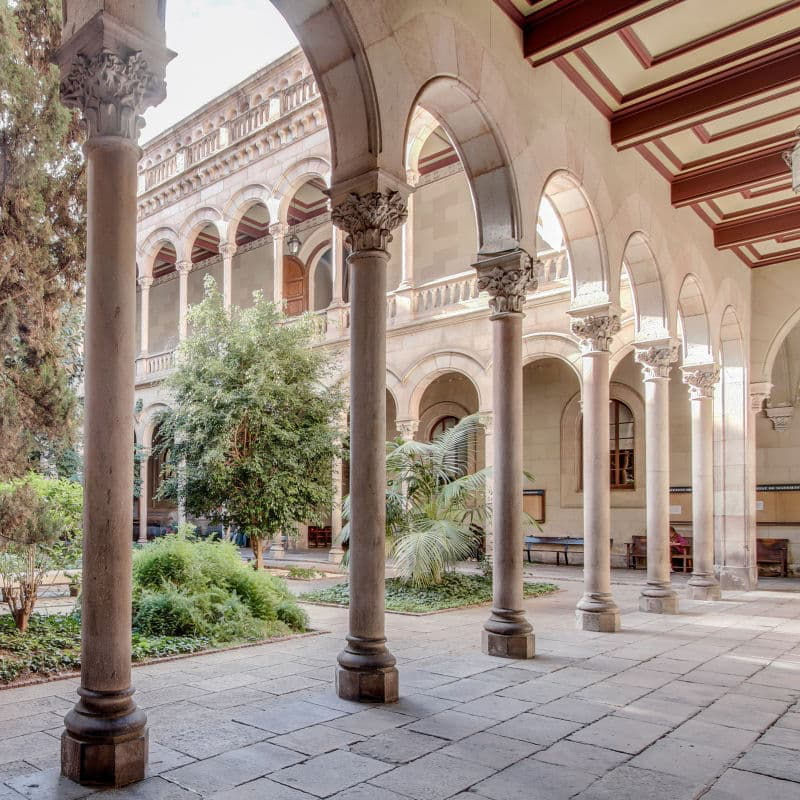
\includegraphics[width=6cm, height=4cm]{images/edifici-historic-universitat-de-barcelona.jpg}
  \end{minipage}
  \begin{minipage}{0.45\textwidth}
    \centering
    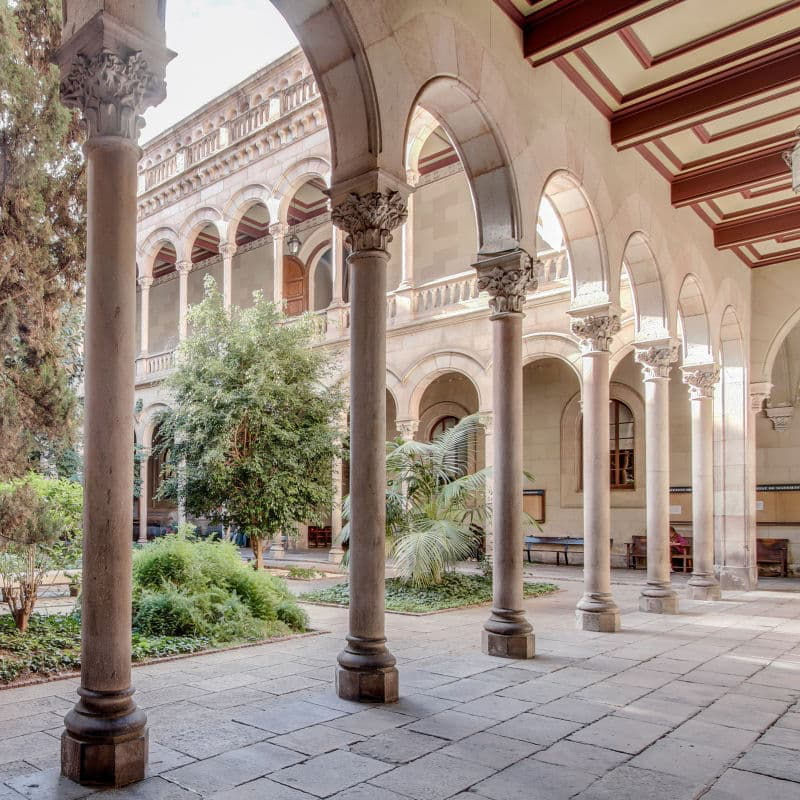
\includegraphics[width=6cm, height=4cm]{images/edifici-historic-universitat-de-barcelona.jpg}
  \end{minipage}
  \caption{Caption for both figures}
  \label{fig:two_images}
\end{figure}


\textbf{Example of the use of the label:} \\
As you can see in the Figure \ref{fig:two_images}, there are two pictures but only one caption, also it is in the page \pageref{fig:two_images}.


\textbf{Example of wrapping the text around the figure:}\\

\begin{wrapfigure}{r}{0.25\textwidth} %this figure will be at the right
    \centering
    
\includegraphics[width=0.25\textwidth]{preambles/static/ub_logo/ub_logo_3.png}
\end{wrapfigure}
The University of Barcelona (Catalan: Universitat de Barcelona, UB; Spanish: Universidad de Barcelona) is a public university located in the city of Barcelona, Catalonia, in Spain. With 63,000 students, it is one of the biggest universities in Spain. It is one of the oldest universities in both Catalonia and Spain, established in 1450.
It is considered one of the best universities in Spain. Overall, the UB has been ranked 1st in Spain in most of the 2022-2023 rankings and is located around the 50th place in Europe. 


\begin{wrapfigure}{l}{0.35\textwidth}
    \centering
    
\includegraphics[width=0.35\textwidth]{preambles/static/ub_logo/ub_logo_1.png}
\end{wrapfigure}
It has 106 departments and more than 5,000 full-time researchers, technicians and research assistants, most of whom work in the 243 research groups as recognized and supported by the Government of Catalonia. 

In 2010, the UB was awarded 175 national research grants and 17 European grants and participated in over 500 joint research projects with the business sector, generating an overall research income of 70 million euros. 

The work of these groups is overseen by the UB's research centres and institutes which collaborate with leading research institutions and networks in Spain and abroad. 

\let\clearpage\relax        %% This command prevents the list of figures to start in a new page
\listoffigures

\newpage




\newpage



\section{Math example}

Example math equation on the sentence:

The most famous equation in the world: $E^2 = (m_0c^2)^2 + (pc)^2$, which is 
known as the \textbf{energy-mass-momentum} relation as an in-line equation.


Example math equation on the squart:

\begin{equation}
P_{R_X} = P_{T_X} \cdot G_{T_X}  \cdot G_{R_X} \cdot \left( \frac{\lambda}{4\pi d} \right)^2  \cdot \eta
\end{equation}

\section{Table example}

\begin{table}[H]
\caption{A badly formatted table}
\centering
\label{table:bad_table}
\begin{tabular}{|l|c|c|c|c|}
\hline 
& \multicolumn{2}{c}{Species I} & \multicolumn{2}{c|}{Species II} \\ 
\hline
Dental measurement  & mean & SD  & mean & SD  \\ \hline 
\hline
I1MD & 6.23 & 0.91 & 5.2  & 0.7  \\
\hline 
I1LL & 7.48 & 0.56 & 8.7  & 0.71 \\
\hline 
I2MD & 3.99 & 0.63 & 4.22 & 0.54 \\
\hline 
I2LL & 6.81 & 0.02 & 6.66 & 0.01 \\
\hline 
CMD & 13.47 & 0.09 & 10.55 & 0.05 \\
\hline 
CBL & 11.88 & 0.05 & 13.11 & 0.04\\ 
\hline 
\end{tabular}
\end{table}



\begin{table}[H]
\caption{A nice looking table}
\centering
\label{table:nice_table}
\begin{tabular}{l c c c c}
\hline 
\multirow{2}{*}{Dental measurement} & \multicolumn{2}{c}{Species I} & \multicolumn{2}{c}{Species II} \\ 
\cline{2-5}
  & mean & SD  & mean & SD  \\ 
\hline
I1MD & 6.23 & 0.91 & 5.2  & 0.7  \\

I1LL & 7.48 & 0.56 & 8.7  & 0.71 \\

I2MD & 3.99 & 0.63 & 4.22 & 0.54 \\

I2LL & 6.81 & 0.02 & 6.66 & 0.01 \\

CMD & 13.47 & 0.09 & 10.55 & 0.05 \\

CBL & 11.88 & 0.05 & 13.11 & 0.04\\ 
\hline 
\end{tabular}
\end{table}


It high recommended to use {\url{https://www.tablesgenerator.com/#}} to generate easy table.




\chapter{My third chapter}

Write your conclusion here.






\chapter{Glossary tutorial}

 The \Gls{latex} typesetting markup language is specially suitable 
for documents that include \gls{maths}. Give



\chapter{bibliograp Tutorial}

Using you can display a bibliography divided into sections, depending on citation type. 
Let's cite! Einstein's journal paper \cite{einstein} and Dirac's book \cite{dirac} are physics-related items. 
Next, \textit{The \LaTeX\ Companion} book \cite{latexcompanion}, Donald Knuth's website \cite{knuthwebsite}, \textit{The Comprehensive Tex Archive Network} (CTAN) \cite{ctan} are \LaTeX-related items; but the others, Donald Knuth's items, \cite{knuth-fa,knuth-acp} are dedicated to programming.



\chapter{Exanple of Indices of terms}

In this example, several keywords\index{keywords} will be 
used which are important and deserve to appear in the 
Index\index{Index}.

Terms like generate\index{generate} and some\index{others} 
will also show up. Terms in the index can also be 
nested \index{Index!nested}  % tutorial, before start, delete it



%% ******************* Contents ********************* %%

\chapter{Here begins your story..}

...

%% ******************* Contents ********************* %%



%% ******************* optional zone ******************* %%

\printbibliography[
heading=bibintoc,
title={Bibliography}
]

\include{optional/references/references}
\appendix

\begin{appendices}
    
\chapter{An example of an appendix}

This is what an appendix looks like!
    
\chapter{LICENSE}
%% This shows appendix shows how to attach a file to the appendix.

MIT LICENSE
    %....
    
\end{appendices}
%% Indices of alphabetic list containing the main terms.
%% tutorial && example:
%% https://www.overleaf.com/learn/latex/Indices   


%% \index{contents}
%% example:
%In this example, several keywords\index{keywords} will be 
%used which are important and deserve to appear in the 
%Index\index{Index}.

%Terms like generate\index{generate} and some\index{others} 
%will also show up. Terms in the index can also be 
%nested \index{Index!nested}



\clearpage
\printindex




%% ******************* optional zone ******************* %%




\end{document}

